\documentclass[12pt,a4paper]{article}
\usepackage[utf8]{inputenc}
\usepackage[margin=1in]{geometry}
\usepackage{graphicx}
\usepackage{float}
\usepackage{amsmath}
\usepackage{listings}
\usepackage{xcolor}
\usepackage{algorithm}
\usepackage{algpseudocode}
\usepackage{enumitem}
\usepackage{tikz}

% Code listing style
\lstset{
    language=C++,
    basicstyle=\ttfamily\footnotesize,
    keywordstyle=\color{blue},
    commentstyle=\color{green},
    stringstyle=\color{red},
    numbers=left,
    numberstyle=\tiny,
    frame=single,
    breaklines=true
}

\begin{document}

% Front Page
\begin{titlepage}
  \centering
  \vspace*{3cm}

  {\Huge\bfseries CSE 406 – Lab Report 3: Round Robin (RR) Scheduling Algorithm \par}
  \vspace{2.5cm}

  \noindent
  \begin{minipage}[t]{0.48\textwidth}
    {\large\bfseries Submitted By:}\\[0.5em]
    \Large
    Sharif Md. Yousuf \\
    ID: 22101128 \\
    Section: C-2 \\
    4th Year, 1st Semester \\
    Spring 2025
  \end{minipage}
  \hfill
  \begin{minipage}[t]{0.48\textwidth}
    {\large\bfseries Submitted To:}\\[0.5em]
    \Large
    Atia Rahman Orthi \\
    Lecturer \\
    Department of Computer Science \& Engineering \\
    University of Asia Pacific
  \end{minipage}

  \vfill

  {\Large\bfseries Date of Submission:} \\[0.5em]
  {\LARGE\bfseries 29 July, 2025 (Tuesday)}

  \vspace*{2cm}
\end{titlepage}

\section{Problem Statement}
I need to implement the Round Robin CPU scheduling algorithm to fairly distribute CPU time among multiple processes. In this algorithm, each process gets a small unit of CPU time called a time quantum, and if a process doesn't complete in that time, it's put back at the end of the queue to wait for another turn.

For this lab, I'm using the following sample case:

\begin{verbatim}
5 2
P1 0 5
P2 1 3
P3 2 1
P4 3 2
P5 4 3
\end{verbatim}

Where the first line contains the number of processes (5) and the time quantum (2), and each subsequent line contains the process ID, arrival time, and burst time.

\section{Objective}
In this lab, I wanted to:
\begin{itemize}
    \item Create my own implementation of the Round Robin scheduling algorithm
    \item See how the time quantum affects process execution
    \item Calculate important metrics like completion time, turnaround time, and waiting time
    \item Understand how processes share CPU time fairly
    \item Get hands-on experience with a preemptive scheduling technique
\end{itemize}

\section{Source Code Screenshot}
\begin{figure}[H]
    \centering
    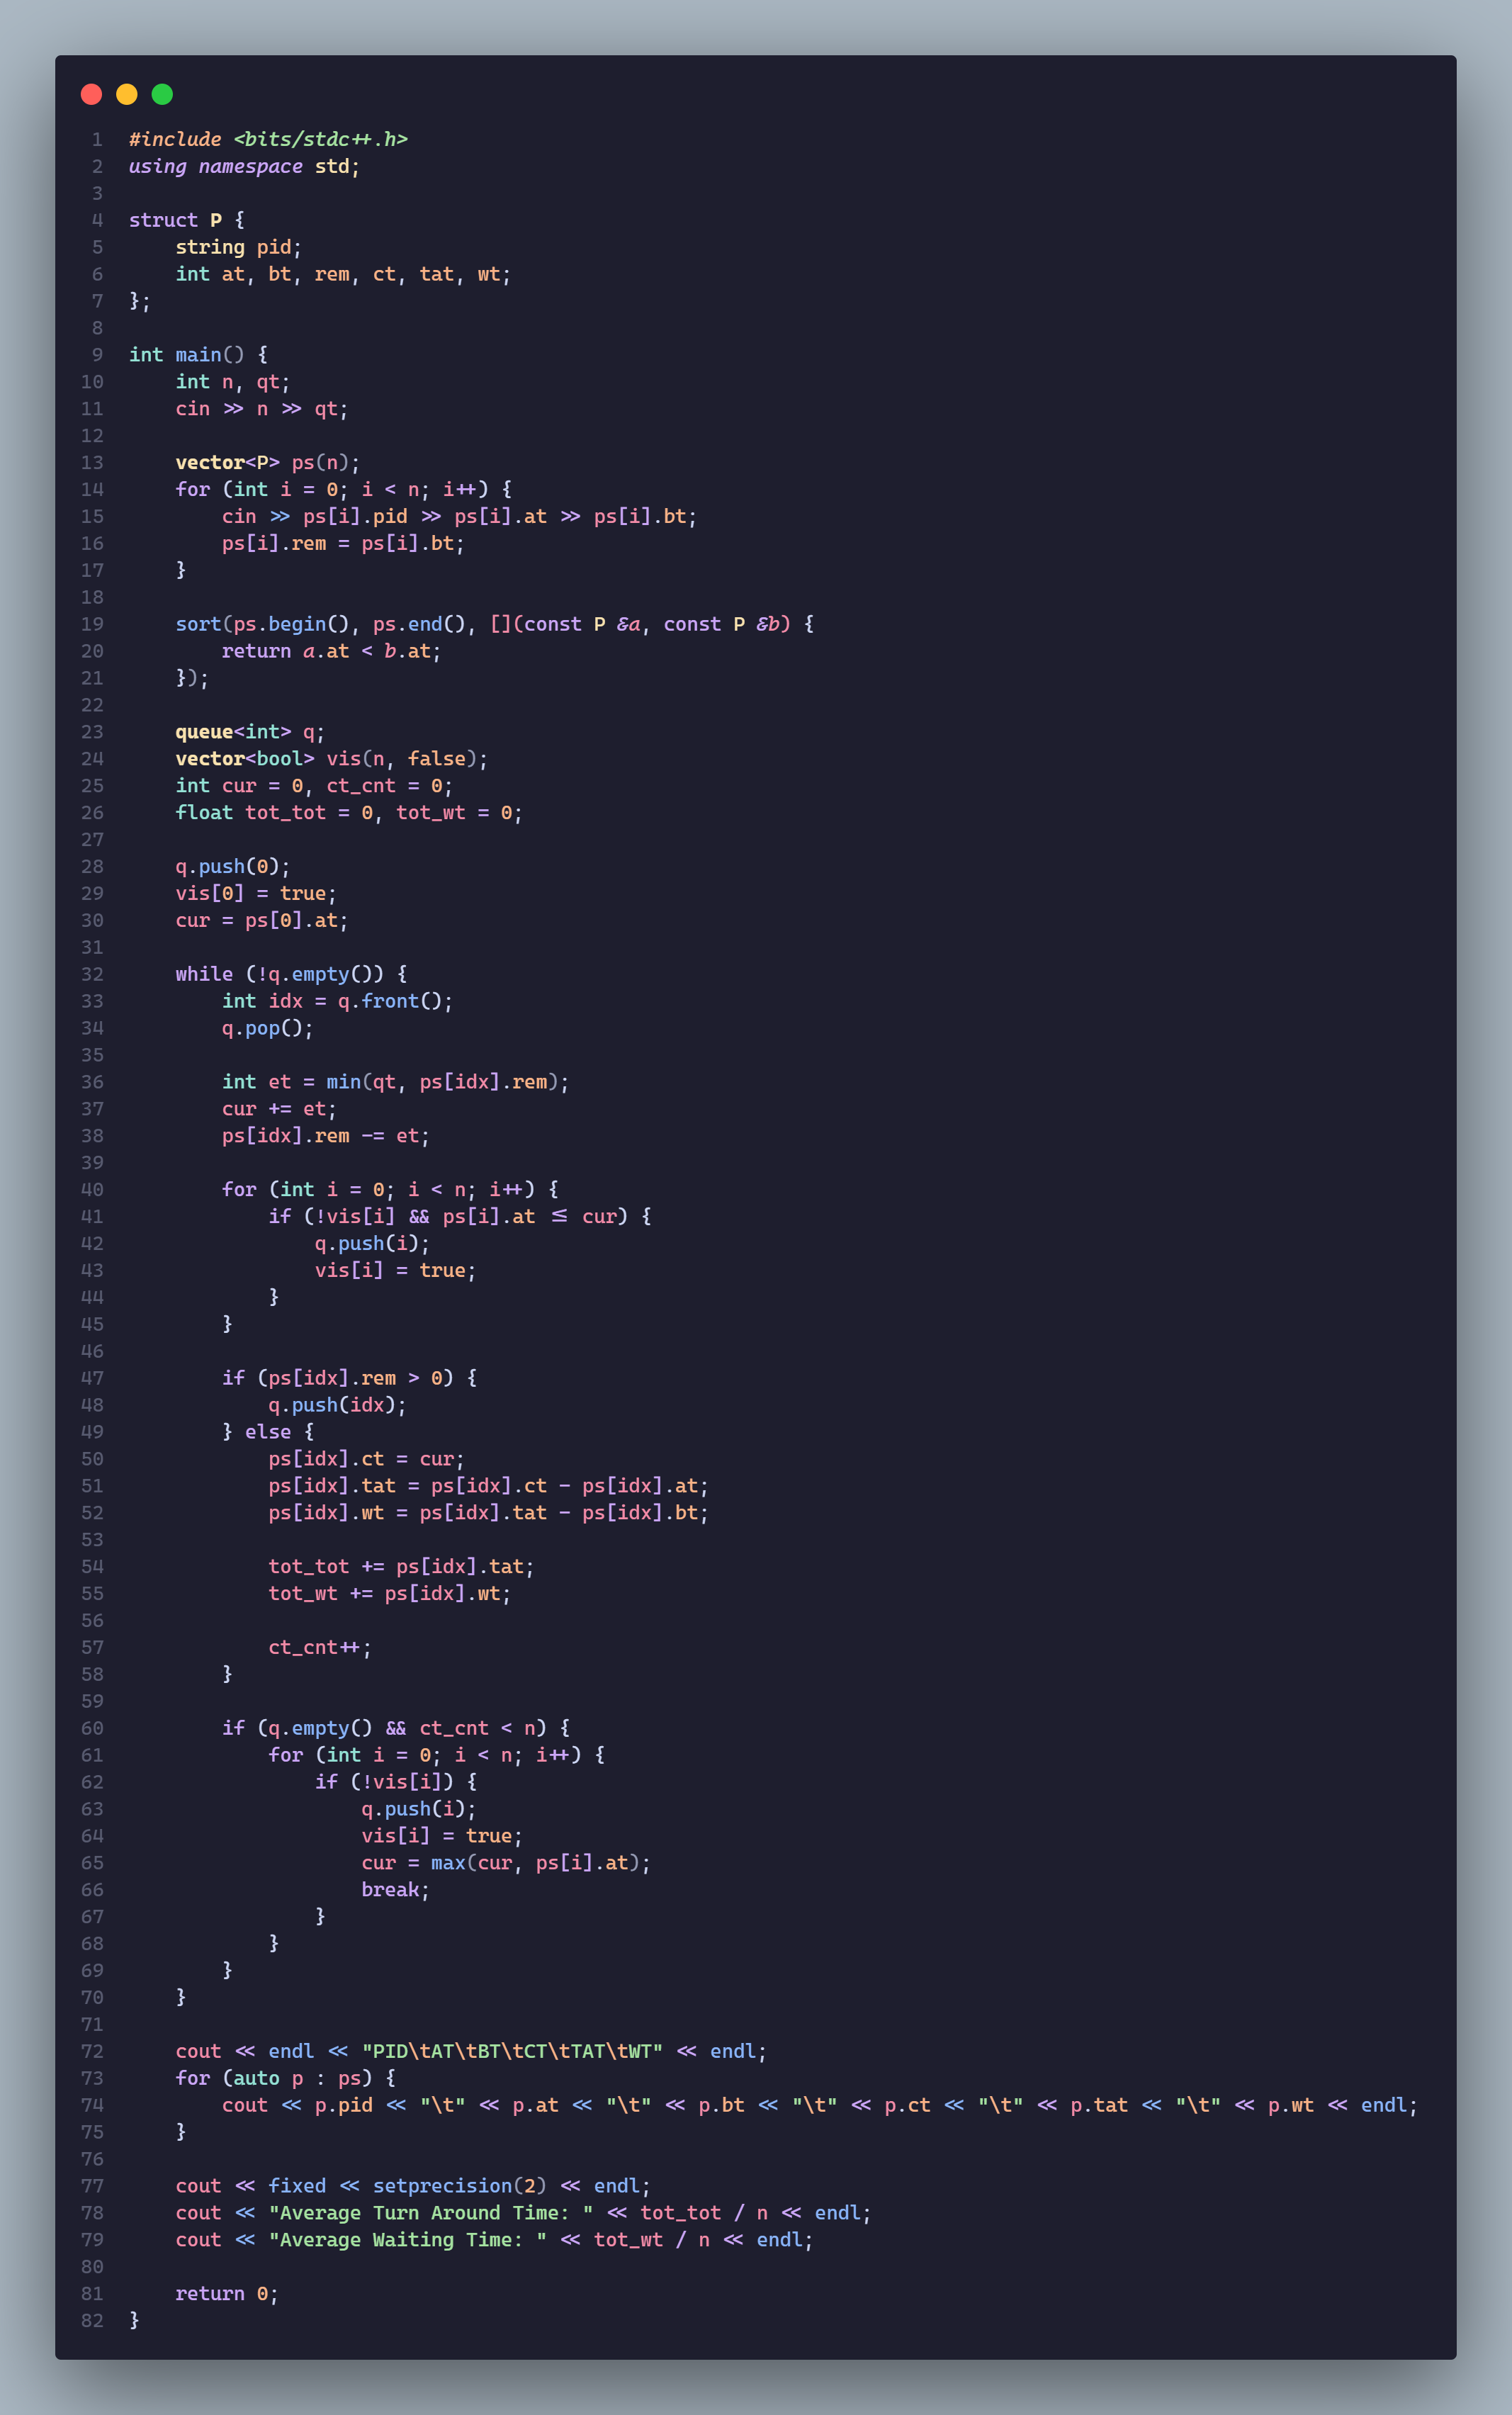
\includegraphics[width=0.9\textwidth]{code.png}
    \caption{Round Robin C++ Code Implementation}
    \label{fig:code}
\end{figure}

\section{Output Screenshot}

\begin{figure}[H]
    \centering
    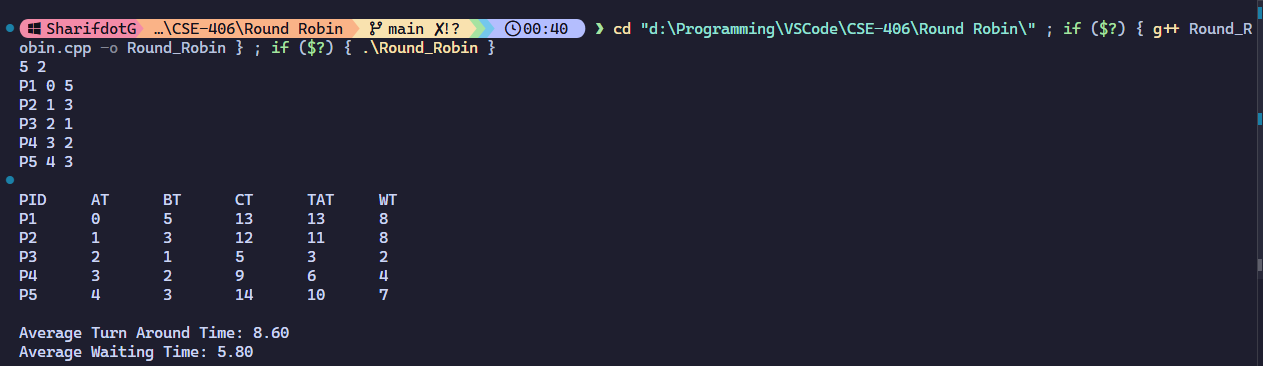
\includegraphics[width=0.9\textwidth]{Screenshot 2025-07-29 004149.png}
    \caption{Output of Round Robin Algorithm Execution}
    \label{fig:output}
\end{figure}

As you can see from the output above, I ran the program with 5 processes and a time quantum of 2. The results show how each process was handled:

\begin{itemize}
    \item Process P1 arrived at time 0, needed 5 time units, and finished at time 13
    \item Process P2 arrived at time 1, needed 3 time units, and finished at time 12
    \item Process P3 arrived at time 2, needed just 1 time unit, and finished quickly at time 5
    \item Process P4 arrived at time 3, needed 2 time units, and finished at time 9
    \item Process P5 arrived at time 4, needed 3 time units, and finished at time 14
\end{itemize}

The average turnaround time came to 8.60 time units, and the average waiting time was 5.80 time units.\section{Discussion}
Working with the Round Robin algorithm was really interesting! Here's what I learned:

The key thing about Round Robin is how it gives each process a fair shot at running. No process can hog the CPU for too long, which means that even if a long process comes in early, shorter processes that arrive later don't have to wait forever.

I found that the time quantum (2 units in my example) really matters:
\begin{itemize}
    \item If it's too small, the system spends too much time switching between processes
    \item If it's too large, it starts behaving more like a first-come-first-served system
    \item Finding the ``sweet spot'' depends on the types of processes you're running
\end{itemize}

My implementation used a queue to keep track of which process should run next, along with a visited array so I wouldn't add the same process to the queue multiple times. This made sure everything ran smoothly.

One cool thing about Round Robin is how responsive it feels. Shorter processes get completed relatively quickly since they don't have to wait for long processes to finish completely before getting CPU time.

\section{Conclusion}
Overall, this Round Robin scheduling lab was really valuable! I got to see firsthand how a time-sharing system works and why it's so important in modern operating systems.

The most important takeaway for me was understanding the tradeoff between fairness and efficiency. Round Robin might not always give the absolute fastest average turnaround time, but it makes sure every process gets its fair share of attention.

I also learned that implementation details matter --- using the right data structures (like queues) and handling special cases (like CPU idle time) can make a big difference in how well the algorithm performs.

If I were to expand on this project in the future, I might try implementing different time quantum values to see how they affect performance, or maybe add process priorities so that more important processes get more frequent turns.

This lab helped me understand why Round Robin scheduling is still widely used in modern operating systems and time-sharing systems --- it's a simple but powerful approach that balances the needs of multiple processes effectively.

\end{document}
